\documentclass[9pt,twocolumn,twoside]{pnas-report}

\templatetype{pnasresearcharticle}

\usepackage{lipsum}

\title{Predicting Popularity of Spotify Playlists from Graph Topology}

\author[a]{Matej Bevec}
\author[a]{Ožbej Pavc} 
\author[a]{Dimitar Nakov}
\author[a]{Jakob Mrak}

\affil[a]{University of Ljubljana, Faculty of Computer and Information Science, Ve\v{c}na pot 113, SI-1000 Ljubljana, Slovenia}

\leadauthor{Jakob, Ožbej, Dimitar, Matej} 
% \authordeclaration{All authors contributed equally to this work.}
% \correspondingauthor{\textsuperscript{1}To whom correspondence should be addressed. E-mail: fine.author@email.com.}

\begin{abstract}
Predicting the virality of music playlists is a task that can have a significant impact on content promotion on platforms like Spotify.
%It involves understanding the underlying structure of user-curated content and its interaction with music artists.
This project investigates the feasibility of predicting whether a playlist is (or will be) viral, i.e., has many followers, only from its structural position within the playlist-track bipartite graph. Leveraging the Spotify Million Playlist Dataset, we construct such a graph and examine various graph-based machine learning models for node-level binary classification. These include graph heuristics, node embeddings, metadata-informed models, and graph neural networks. Given the heavy class imbalance inherent in real-world playlist popularity, we employ multiple data balancing strategies to create workable subgraphs for training and evaluation. While our results suggest that most models struggle to significantly outperform a naive baseline, which confirms our preliminary analysis, the best approaches achieve modest predictive power (up to 67\% accuracy on balanced test sets), highlighting both the difficulty and potential of using network structure alone to forecast playlist success.


% With this project, we aim to assess whether graph topology alone can be used to predict whether a playlist will be viral, based on its connections in a bipartite graph of playlists and artists. We created a graph from a real Spotify playlist dataset, where each node represents a playlist and an artist, and the edges indicate that a track from a given artist is included in the playlist. In terms of evaluation, we used a variety of different models, some of which include: traditional graph-based baselines (e.g., Node2Vec + Logistic Regression, Spectral Embedding), handcrafted descriptors (e.g., Track Degree, Name Embeddings), and more expressive models like Graph Neural Networks (GraphSAGE). The results reported are under a consistent training and evaluation setup, and finally, we conclude with an analysis of performance gaps and opportunities for improvement.
\end{abstract}

\dates{The manuscript was compiled on \today}
\doi{\href{https://ucilnica.fri.uni-lj.si/course/view.php?id=183}{Introduction to Network Analysis} 2024/25}

\begin{document}

\maketitle
\thispagestyle{firststyle}
\ifthenelse{\boolean{shortarticle}}{\ifthenelse{\boolean{singlecolumn}}{\abscontentformatted}{\abscontent}}{}

\section*{Introduction}
Playlists play a crucial role in music discovery, recommendation, and curation, and they especially have a great impact on artists, listeners, and platform designers. As such, the capability to predict how popular a Spotify playlist is (or will be) has great commercial value. 
In this project, we attempt a challenging task to predict a playlist's popularity (measured by follower count) using only its position and structure within the Spotify playlist-track bipartite graph.
This is a task in the field of graph-based machine learning, where network topology is used to model and predict node-level attributes. As input, we take a bipartite playlist-track graph where playlists and tracks are nodes, and an edge exists if the given track is in the given playlist.
We explore a myriad of node classification models, including: simple graph-based heuristics, transductive node embeddings, node-descriptor-based approaches, and graph neural networks (GNN). These models serve as great baselines for evaluating the predictive power of local topology. We aim to benchmark multiple approaches under a unified evaluation framework to better understand how well different aspects of graph structure capture the notion of virality.

This project represents a structured and empirical foundation for using graph-based models to predict playlist success, giving insight into the relationship between network structure and user engagement on music platforms.

\section{Dataset}
We used the Spotify Million Playlist Dataset (MPD), originally released as part of the RecSys Challenge 2018 \cite{aicrowd}. The dataset contains one million public playlists created by U.S.-based Spotify users between January 2010 and November 2017. It includes over two million unique tracks and approximately 300,000 different artists. Each playlist entry provides its unique ID, name, track list, number of followers, and the creation timestamp. For each track, additional metadata such as track name, artist, and album information is included. An accessible copy of the dataset is also available on Kaggle \cite{kaggle}.


\section{Data Preparation and problem framing}
\label{sec:prep}


\begin{figure}[htbp]
    \centering
    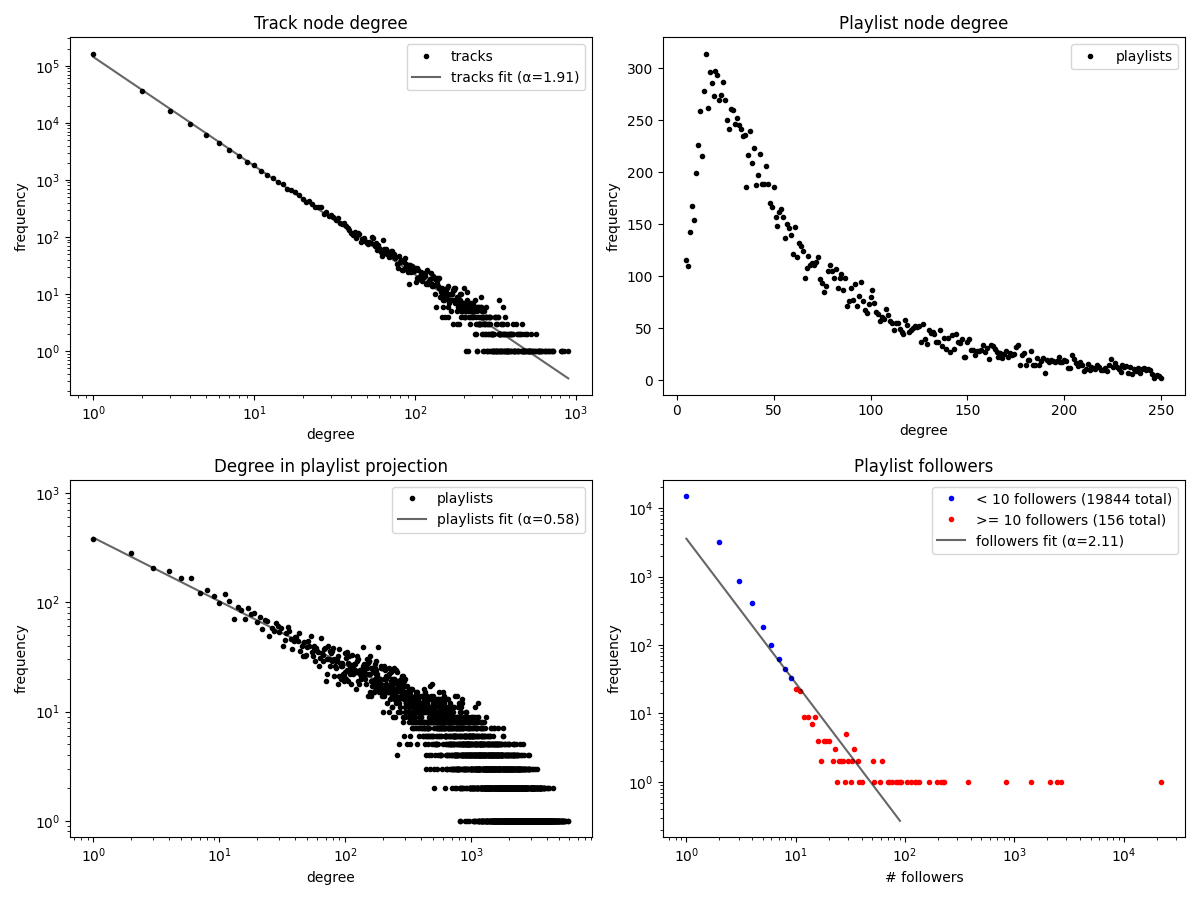
\includegraphics[width=0.5\textwidth]{fig/distributions_uniform_20k.png}
    \caption{Degree and follower distributions for the "uniform 20k" network.}
    \label{fig:dist-u20}
\end{figure}

\subsection{Graph construction}

To represent playlist-track relationships, we build a bipartite graph where one partition contains playlists and the other contains tracks. An edge between a playlist and a track indicates that the track appears in the playlist. This bipartite structure contains no direct links between playlists or between tracks.

\paragraph{}
The track degree distribution is perfectly power-law distributed with an exponent $\alpha = 1.91$ (Figure \ref{fig:dist-u20}) --- some tracks are popular and present in many playlists (hubs), while most are not. 
The playlist degree distribution exhibits a peak followed by an exponential decay to the right. It appears that there is a mean playlist length (approx. 25 in the \textit{uniform 20k} dataset), but some playlists are significantly longer.

The dataset is characterized by a highly skewed follower distribution, which follows a heavy-tailed power-law ($\alpha > 2.1$) --- most playlists have no followers, while a few attain tens of thousands. In fact, only about $0.8\%$ have over 10!
Such distributions are common in social and recommender systems, but they pose challenges for standard classification approaches.

\subsection{Binary classification and distribution skew}
For our task, we consider the \textit{playlist-track bipartite graph} as our input, individual playlist nodes as samples, and their follower count as our quantitative target variable.
Additionally, some models may use \textit{node metadata} or the \textit{playlist-projection graph}, where playlist nodes are connected if they share tracks.

Since our goal is to tell a user whether their playlist will be popular or not, we deem it most sensible to frame our task as a binary classification task. We define a playlist with at least \textit{10 followers to be viral or popular, while the rest are non-viral or unpopular}. 

In this setup, the extremely skewed follower distribution presents a significant challenge. For example, in a uniformly-sampled network subset with 20 thousand playlists and almost x tracks (Figure \ref{fig:dist-u20}), only 120 playlists fall under "viral". Models trained on the full dataset without adjustment
quickly learn to predict the dominant class ("unpopular") to minimize loss, and may fail to identify rare but important viral playlists.

To address this, we balance the set of training samples --- the "viral" set remains the same while the "non-viral" set is subsampled to match its size. This means the models only see targets for these samples during training, \textit{but otherwise use the entire network for analysis}.

\subsection{Balancing the dataset}

Unfortunately, this introduces another issue. On the one hand, subsampling of the majority class yields a very small training set compared to the scale of the model. On the other hand, our choice to evaluate, along with more scalable methods, transductive methods that require the entire graph to be present in memory, limits us to relatively small subgraphs of the full network. This leaves us with very few training samples.

To address this, we take two approaches:
\begin{itemize}
    \item \textbf{Class-balanced network.} We subsample the majority class to match the minority class and induce a subgraph on the selected nodes. Even though this might introduce biases into the network structure, it gives us a much larger training set relative to network size, since the training samples now span all nodes. With this approach, we prepare a network with 5k nodes (and 5k train+test samples) for training.
    \item \textbf{Uniformly sampled network.} We uniformly sample nodes to get a graph of the desired size, but try to combat the scale and the lack of samples in different ways. Since the projection graph is most problematic due to its many edges, we reduce its size only connecting playlists if they share at least 3 tracks. Additionally, we upsample the minority class by simply duplicating all samples 5 times, before balancing the majority class. With a somewhat higher risk of overfitting, we now have 5x more information about the non-viral playlists, but not about viral playlists. With this approach, we prepare a 5k playlists variant to match the balanced dataset (this equates to only 520 train+test samples), and a 20k variant to obtain at least the same order of magnitude of samples (1560).
\end{itemize}


% The Million Playlist Dataset exhibits extreme imbalance in follower counts—most playlists have zero followers, while only a small fraction become popular. To mitigate this, we implemented two sampling strategies.

% In the first, called \textit{balanced sampling}, we created a binary dataset where playlists with at least 10 followers were labeled as popular. We then uniformly sampled from the much larger group of unpopular playlists to create a balanced dataset. This allowed classifiers to be trained without overwhelming bias toward the majority class.

% In parallel, we also prepared a version based on \textit{uniform sampling}, in which playlists were sampled randomly regardless of their popularity. This variant preserved the natural distribution of follower counts and allowed for realistic evaluation of model performance on skewed data.

% \subsection{Graph Construction}
% To represent playlist-track relationships, we built a bipartite graph where one partition contains playlists and the other contains tracks. An edge between a playlist and a track indicates that the track appears in the playlist. This bipartite structure contains no direct links between playlists or between tracks.

% We then projected this bipartite graph onto the playlist side, connecting two playlists if they share at least one track. The resulting unipartite graph has weighted edges, where edge weight corresponds to the number of shared tracks. These projected graphs were the foundation for extracting structural network descriptors and constructing feature matrices for our models.

% \section{Distribution Skew}
% A key property of the dataset is its highly imbalanced follower distribution, which follows a heavy-tailed power-law. Most playlists have no followers, while a few attain tens of thousands. Such distributions are common in social and recommender systems, but they pose challenges for standard classification approaches.

% Models trained on the full dataset without adjustment quickly learn to predict the dominant class ("unpopular") and may fail to identify rare but important viral playlists. Moreover, conventional metrics such as accuracy or F1 score can be misleading, as high performance can be achieved by simply predicting the majority class.

% To address this, we relied on data balancing and used robust evaluation metrics such as precision, recall, and area under the PR curve. Additionally, we visualized the follower distribution to better understand the severity of class imbalance and its implications for modeling.


\section{Preliminary Analysis}
Initially, for achieving our goal of predicting playlist popularity, we tried calculating some graph features. These were then used to visualize their relationship and correlation with the number of playlist followers. Note that these analyses are performed over all nodes in the graph and not just the balanced training set described in \ref{sec:prep}.

\subsection{Graph Feature Extraction}
For each graph, we computed quite a few metrics: Degree, Closeness centrality, Betweenness centrality, Katz centrality, Eigenvector centrality, and Clustering coefficient. Some of them can be computed fast by using the networkx library \cite{networkx} (like degree), but others require more time. Therefore, we sped up the process by computing some features using a GPU-accelerated library cuGraph \cite{cugraph}. However, for example clustering coefficient does not have a GPU-accelerated algorithm, and there we used the library igraph \cite{igraph}, which is supposedly faster than networkx.

\subsection{Binary Threshold Evaluation}
Using metrics like precision, recall, F1, AUC, etc., we better understood the importance of the relation between playlist popularity and graph topology. We calculated these metrics for multiple feature thresholds on balanced and uniform graphs. One of the metrics and visualizations we use is the ROC (Receiver Operating Characteristic) curve, which suggests that such features do not contribute to playlist popularity. This is also shown in the following plot \ref{fig:roc}.

\begin{figure}[htbp]
\centering
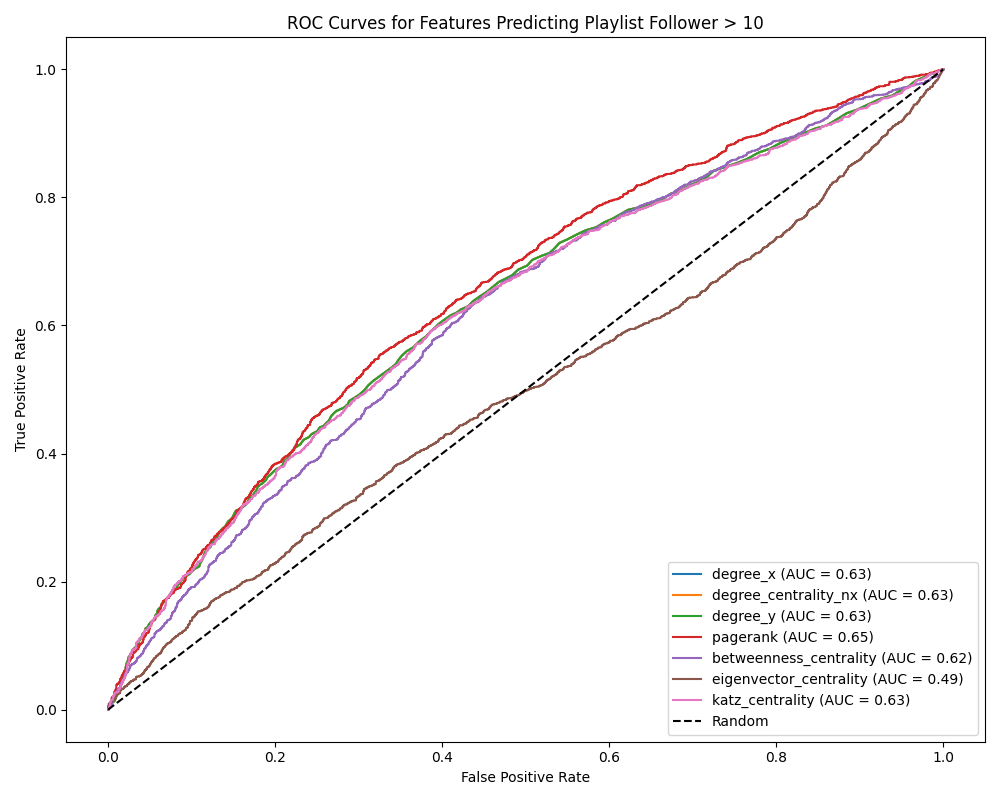
\includegraphics[width=0.45\textwidth]{fig/roc_plot.png}
\caption{ROC curves for selected descriptors computed on balanced sampled 5k playlist graph}
\label{fig:roc}
\end{figure}

\subsection{Correlation with Followers}
To further evaluate the correlation between features and playlist follower count, we computed Spearman and Kendall correlation. As binary threshold evaluation already suggested, the correlation values showed little correlation between many calculated features. Using a projected version of graphs (ex. figure \ref{fig:correlation}) we found betweenness centrality to be mostly correlated with graph features.

\begin{figure}[htbp]
\centering
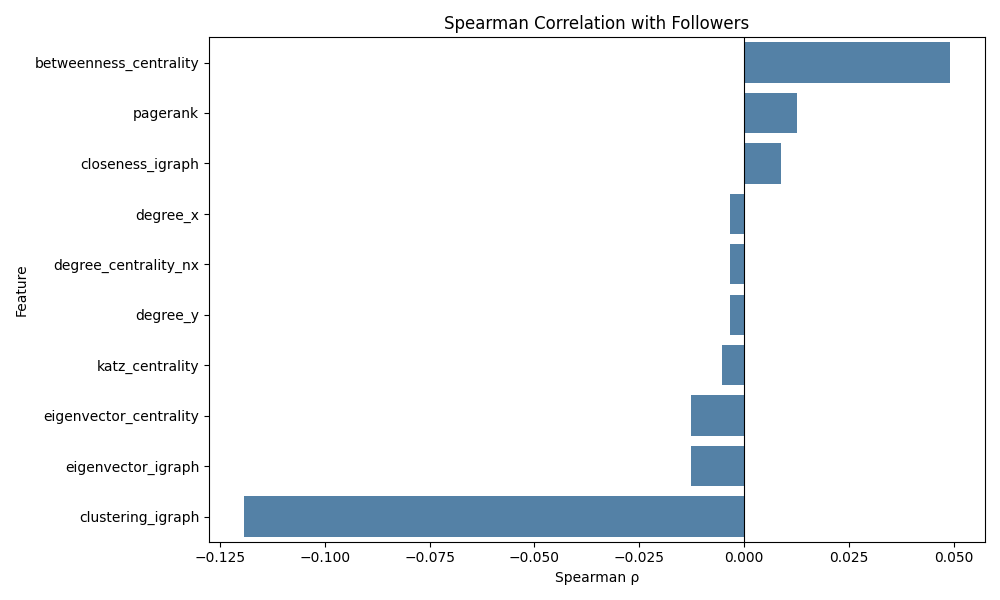
\includegraphics[width=0.45\textwidth]{fig/correlation_plot.png}
\caption{Spearman correllation between features and followers (using 5k playlist subsampled) suggesting little correlation or none at all}
\label{fig:correlation}
\end{figure}

\subsection{Community Detection}
One more idea we had consisted of applying community detection algorithms on our graphs and trying to use communities as possible identifiers of popularity. This however quickly showed that popular and unpopular playlists are not separated into different communities, with bigger communities having half popular and half unpopular ones. Applying the Louvain algorithm resulted in the following figure \ref{fig:community}. Here we see that only the first 6 bins have more than 5 nodes per community. Having a closer look at those, we see them averaging between 0.4 and 0.6 proportion of popular-unpopular playlists. Consequently, this most likely shows that communities are not correlated with the popularity of playlists.

\begin{figure}[htbp]
\centering
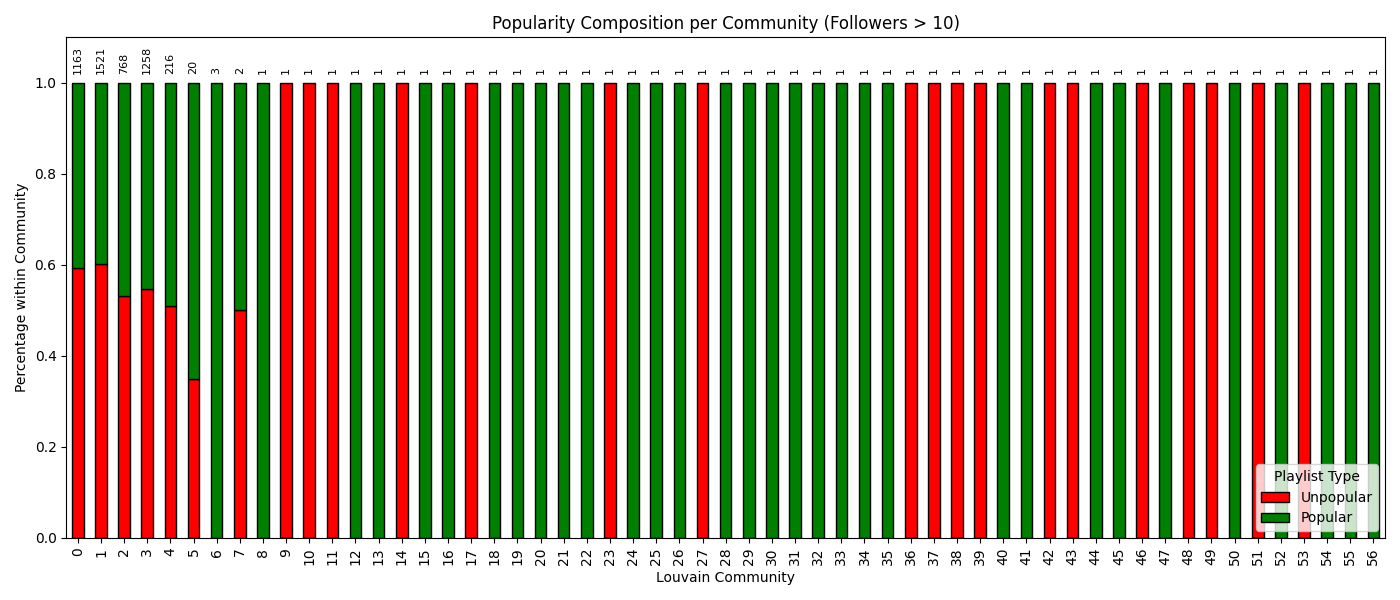
\includegraphics[width=0.45\textwidth]{fig/community_plot.png}
\caption{Proportion of viral playlists per community (on 5k playlist balanced sampled graph)}
\label{fig:community}
\end{figure}

\section{Models}
\subsection{Baselines}
\begin{itemize}
    \item \textbf{Majority classifier:} always predicts the majority class.
    \item \textbf{Track-degree + Logistic regression (LR):} for a given playlist, takes the sum of the degrees of all its neighbors (tracks) as a scalar feature and trains a Logistic regression classifier to predict the target. This feature is used as a proxy for total track "popularity" in a playlist, which may be correlated with the popularity of the playlist itself. Logistic regression is chosen here, and in other models, as the classifier due to its ability to find a signal in a feature space in an efficient manner without significant parameter tuning.
    \item \textbf{Neighbor mean:} for a given playlist, takes the average follower count among its playlist-projection neighbors (playlists that share tracks) and thresholds it to predict the target.
    \item \textbf{Similar neighbor:} for a given neighbor, finds $k$ playlistist with which it shares most tracks. Among those, it takes the maximum follower count and thresholds it to predict the target. If at least one of the very similar playlists is popular, this one may be too.
\end{itemize}

\subsection{Embedding Models}
\begin{itemize}
    \item \textbf{Name embeddings + LR:} playlist names are embedded into 384-feature vectors with \textit{all-MiniLM-L6-v2}, a minified BERT-adjacent sentence transformer trained for general use, such as semantic search. Logistic regression is again used as the classifier. This is a baseline that uses node features only and may reveal whether simple metadata might carry more information about popularity than the network itself.
    \item \textbf{Spectral projection + LR:} the playlist projection graph is embedded with spectral projection, followed by an LR classifier.
    \item \textbf{Node2Vec + Logistic Regression:} the network is embedded with node2vec, followed by an LR classifier. Node2Vec is chosen for its capability to capture both local and global structural patterns in the playlist–track bipartite graph through biased random walks.
    We used Node2Vec with standard hyperparameters (p=1, q=0.5, 128 dimensions) to capture both local and global topological features of the graph.
\end{itemize}

\subsection{GraphSAGE}
Graph neural networks learn representations by aggregating information from neighboring nodes through message passing and may be effective, especially when incorporating node features, at finding complex relationships in graph structure, which our task may require.

We specifically evaluate GraphSAGE \cite{hamilton2017inductive}: an inductive GNN variant, which aggregates a node's neighborhood as follows:
\begin{itemize}
    \item Aggregate neighboring nodes' features, e.g., via a mean
    \item Concatenate with the given node's features
    \item Transform via weight matrix and apply non-linearity
\end{itemize}
We use two convolutional layers --- the first convolution aggregates information from two-hop neighbors to direct neighbors (playlists to tracks), and the second maps from the direct neighbors to the given node (tracks to playlist). This is followed by a dense classification layer. 
The model is trained directly on the classification task using the Adam classifier with BCE loss for 30 epochs.
When it comes to node features, we test three variants. The first uses random initializations (featureless baseline). In the second, node degree is added to the random vectors for all nodes. In both cases, feature vectors are 16-dimensional. In the third, playlist nodes are represented by a 384-feature \textit{all-MiniLM-L6-v2} embedding of the playlist names, while track node features are random with the same size.


\subsection{Node descriptors + NN}
We also evaluate a standard feedforward neural network that uses node descriptors as input features. The input features for each playlist node are derived from a set of metrics, including:
\begin{itemize}
    \item Graph centrality measures (PageRank, betweenness, closeness, clustering coefficient)
    \item Track-based statistics (e.g., average track degree, mean and standard deviation of track frequency, track diversity entropy, average track IDF)
    \item Playlist-level properties (number of tracks - degree, average track duration, common/rare tracks ratio, track diversity measures, and number of unique albums)
\end{itemize}
All features are scaled using a standard scaler, and we filter out non-predictive or redundant fields such as names and identifiers.

The architecture includes three hidden layers (128, 64, 32) with batch normalization, ReLU activations, and dropout (0.4), followed by a final linear layer for binary classification. We train the model using AdamW with cross-entropy loss and a OneCycle learning rate schedule for 200 epochs. The model is evaluated using accuracy, F1 score, recall and precision. 



\paragraph{Note on transductive models:} models like node2vec and spectral embedding are transductive - the entire graph has to be embedded at once - and as such aren’t exactly applicable to our goal task of predicting virality of a newly added playlist node. Still, we evaluate them as baselines.

\paragraph{Note on label-awareness:} while most of our models are trained to classify playlists solely given graph topology (and potentially node features), our task definition allows another information source. When classifying a new node, the target labels (follower counts) of existing nodes are available. Two baselines - Similar Neighbors and Neighbor Mean - make use of this information.


\section{Evaluation}

All models are evaluated on a 70\%/30\% stratified train/test split. Both the train and test are balanced in terms of majority/minority class at appr. 50\%. In the \textit{uniform} datasets, upsampling is performed separately on the train and test sets to avoid leakage. Each model is given the graph and its projection at inference, followed by node indices and corresponding targets during the training step.
We evaluate all models in terms of accuracy, precision, recall, and F1-score with an additional ROC-curve analysis on a raw, unbalanced test set for one of the models.



\section{Results}

\begin{table}[htbp]
\centering
\begin{tabular}{lcccccc}
\toprule
Model & Accuracy & Precision & Recall & F1 \\
\midrule
Majority & 0.509 & 0.509 & 1.000 & 0.000 \\
Track Degree + LR & 0.543 & 0.579 & 0.376 & 0.456 \\
Neighbor mean & 0.503 & 0.507 & 0.969 & 0.665 \\
Similar neighbor (k=5) & 0.511 & 0.510 & 0.996 & 0.675 \\
Name embedding + LR & 0.577 & 0.584 & 0.585 & 0.585 \\
Spectral embedding + LR & 0.510 & 0.510 & 1.000 & 0.675 \\
Node2Vec + LR & 0.56 & 0.58 & 0.53 & 0.55 \\
GraphSAGE (random) & 0.497 & 0.506 & 0.525 & 0.515 \\
GraphSAGE (degree) & 0.597 & 0.613 & 0.567 & 0.589 \\
GraphSAGE (name) & 0.536 & 0.542 & 0.575 & 0.558 \\
Node descriptors + NN & 0.62 & 0.63 & 0.63 & 0.62 \\
\bottomrule
\end{tabular}
\caption{Summary of model performance on the \textit{\textbf{balanced 5k}} network}
\label{tab:res-b5}
\end{table}

\begin{table}[htbp]
\centering
\begin{tabular}{lcccccc}
Model & Accuracy & Precision & Recall & F1 \\
\midrule
Majority & 0.50 & 0.00 & 0.00 & 0.00 \\
Track Degree + LR & 0.56 & 0.56 & 0.56 & 0.56 \\
Neighbor mean & 0.50 & 0.00 & 0.00 & 0.00 \\
Similar neighbor (k=5) & 0.52 & 0.63 & 0.11 & 0.19 \\
Name embedding + LR & 0.48 & 0.42 & 0.11 & 0.18 \\
Spectral embedding + LR & 0.48 & 0.49 & 0.89 & 0.63 \\
Node2Vec + LR & 0.41 & 0.27 & 0.11 & 0.16 \\
GraphSAGE (random) & 0.41 & 0.00 & 0.00 & 0.00 \\
GraphSAGE (degree) & 0.62 & 0.69 & 0.44 & 0.54 \\
GraphSAGE (name) & 0.43 & 0.00 & 0.00 & 0.00 \\
Node descriptors + NN & 0.63 & 0.66 & 0.56 & 0.63 \\

\bottomrule
\end{tabular}
\caption{Summary of model performance on the \textit{\textbf{uniform 5k}} network}
\label{tab:res-u5}
\end{table}

\begin{table}[htbp]
\centering
\begin{tabular}{lcccccc}
Model & Accuracy & Precision & Recall & F1 \\
\midrule
Majority & 0.50 & 0.00 & 0.00 & 0.00 \\
Track Degree + LR & 0.52 & 0.53 & 0.27 & 0.36 \\
Neighbor mean & 0.51 & 0.83 & 0.02 & 0.04 \\
Similar neighbor (k=5) & 0.47 & 0.35 & 0.06 & 0.11 \\
Name embedding + LR & 0.57 & 0.60 & 0.44 & 0.50 \\
Spectral embedding + LR & 0.48 & 0.49 & 0.90 & 0.63 \\
Node2Vec + LR & 0.54 & 0.54 & 0.40 & 0.46 \\
GraphSAGE (random) & 0.49 & 0.49 & 0.27 & 0.35 \\
GraphSAGE (degree) & 0.57 & 0.61 & 0.40 & 0.48 \\
GraphSAGE (name) & 0.48 & 0.40 & 0.10 & 0.17 \\
\bottomrule
\end{tabular}
\caption{Summary of model performance on the \textit{\textbf{uniform 20k}} network}
\label{tab:res-u20}
\end{table}

Looking at the results (tables \ref{tab:res-b5}, \ref{tab:res-u5} and \ref{tab:res-u20}), it is immediately obvious they don't significantly outperform the majority classifiers.
The average popularity of loosely related playlists (Neighbor mean) is not at all an indicator of a given playlist's virality. Taking the most optimistic prediction out of a few very similar playlists (Similar neighbor) expectedly receives a high recall on balanced 5k, but does not discern between good and bad candidates (low accuracy). Surprisingly, recall is not high on other datasets.
\paragraph{}
Neighbors' Track Degree (total song popularity) may encode a very weak signal. Name embeddings at CA at approx. 0.57, node-feature-only Name embeddings outperform many graph-based approaches on the larger datasets, but perform really poorly on the smallest. Perhaps, not enough training samples are available given its relatively large 384-dimensional feature space.
A purely graph-based embedding node2vec performs slightly worse, and similarly underperforms on the smallest network.

\paragraph{}
The second-best baseline is GraphSAGE with node degree features, suggesting that this GNN method is able to aggregate the weak signal in node degree into a meaningful feature set. Less successful are the random and name-embedding variants. In the second case, it seems the track nodes (with random features) may be acting as a barrier in propagating useful information between playlist nodes. 

\paragraph{}
The Node descriptors + NN model achieves the best results --- the NN, with its non-linearity seems to extract a stronger signal from the combination of multiple basic node metrics than the analysis of individual metrics would suggest.






% \begin{figure}[htbp]
% \centering
% 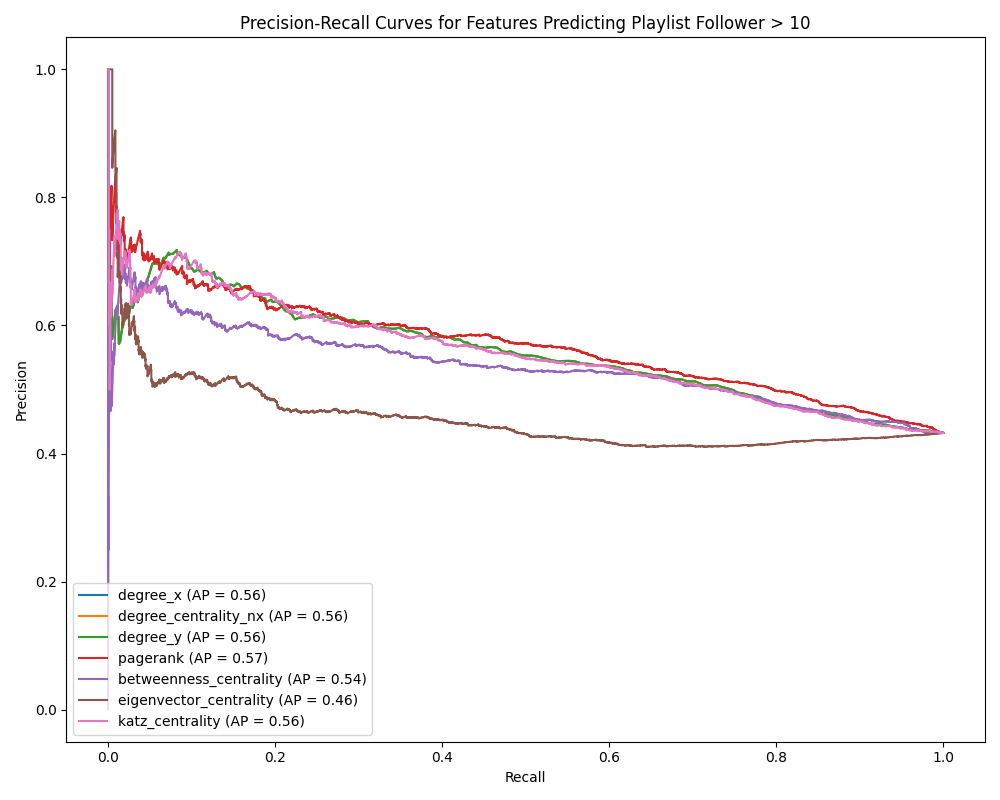
\includegraphics[width=0.45\textwidth]{pr_curves.png}
% \caption{PR curves for selected classifiers}
% \end{figure}

\subsection{Performance on Skewed Data}

\begin{figure}[htbp]
    \centering
    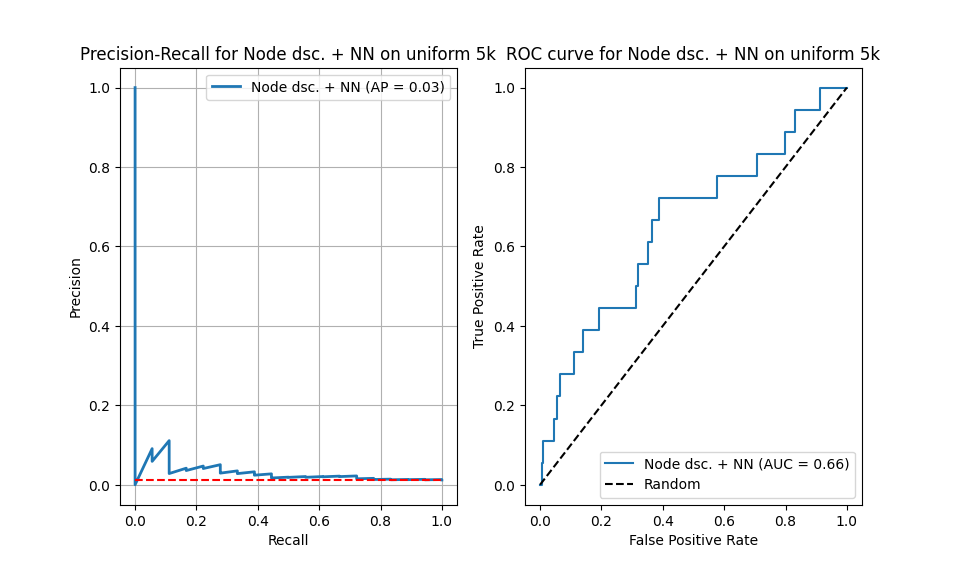
\includegraphics[width=0.5\textwidth]{fig/curves.png}
    \caption{PR and ROC curve for the Node descriptors + NN model on the uniform 5k network with an upsampled balanced training set but a raw unbalanced training set.}
    \label{fig:roc-unbalanced}
\end{figure}

So far, we have evaluated our models on a class-balanced test set. To get a better insight into what the observed results actually mean in a real-life scenario, we analyze the behavior of the best-performing model on a modified variant of the uniform 5k network. Here, the training set remains upsampled and balanced as described in Section \ref{sec:prep}, but the test set is in its raw, unbalanced form -- we simply take all nodes in the 30\% split. 
Figure \ref{fig:roc-unbalanced} shows the ROC and Precision-Recall curves for this setup. Unfortunately, due to a very small number of positive samples, its interpretation might not be very reliable (notice the "jagged" appearance).
Considering the peaks are not overly optimistic, the model threshold could be set at $recall=0.13$ $precision=0.11$ .

\section{Possible Improvements}
\begin{itemize}
    \item Advanced upsampling with GraphSMOTE: other than simple duplication, upsampling of the minority class could be approached with GraphSMOTE, which generates synthetic nodes by perturbing a similarity-encoding node embedding. This could improve performance by ensuring a large but diverse balanced training set.
    \item Scalable methods on larger networks: scalable methods like GraphSAGE should be evaluated on larger datasets (like the original 1M network), possibly improving performance.
    \item Improvements to the GraphSAGE models: while there are many parameters that could be tuned in training and architecture, perhaps skipping tracks in neighbor sampling and performing convolutions playlist to playlist only, would prevent information through track nodes. This could be paired with similarity-based sampling like in PinSage \cite{ying2018graph}.
    \item Incorporating audio or genre features: In our study, we considered only simple node metadata. Augmenting the original graph with e.g., audioclips or genre tags would provide richer node features.
    \item Tripartite graphs with artist-level metadata: new information could be injected into the graph structure by connecting tracks which belong to the same artist and thus adding an artist partition to the network.
    \item Popularity-focused playlist completion: given a well-performing inductive model trained for our task, we could help users create popular playlists. An existing playlist "stem" could be used as a seed to generate similar track recommendations (e.g., PPR visit counts). Then, this set could be filtered to only include tracks that would, according to our model, improve the playlist's "virality". 
\end{itemize}

\section{Conclusion}
Our experiments demonstrate that some models do learn weakly predictive signals for virality prediction from graph structure, though overall performance remains close to baseline in most cases. These findings suggest that while network features contain some information relevant to playlist success, they are likely insufficient on their own for high-accuracy prediction. Future work could explore integrating richer content-based or focus on hybrid models that combine topology with user and track-level metadata to more accurately model playlist popularity dynamics.

\nocite{bevec2025spotify}

% \acknow{The authors would like to\dots}
% \showacknow{}

\bibliography{literature}

\end{document}